\documentclass{fkssolpub}

\usepackage[czech]{babel}
\usepackage{fontspec}
\usepackage{fkssugar}
\usepackage{amsmath}
\usepackage{graphicx}

\author{Ondřej Sedláček}
\school{Gymnázium Oty Pavla} 
\series{FO-B-S}
\problem{2} 

\begin{document} 

Ze vztahu pro magnetickou indukci kolem dlouhého přímého vodiče
$B = \mu \frac{I}{2 \pi d}$ je vidět, že velikost magnetické indukce $B$ 
je nepřímo úměrný vzdálenosti od vodiče $d$. Toho při výpočtech budu
využívat hojně, protože mi to umožňuje vyjadřovat velikost magnetické
indukce jako násobky $B_1$.

Víme, že bod $K$ je vzdálen od druhého vodiče $2r$ a bod $L$ je vzdálen
$4r$. Pro uvážení souhlasného a nesouhlasného směru nám stačí jen prohodit
znaménka pro velikost magnetické indukce vyvolaný druhým vodičem, protože
magnetické indukce prvního a druhého vodiče leží na stejné přímce. Proto
tedy velikosti $B_K$ a $B_L$ vypočítáme jako:

\[
  B_K = |B_1 \mp \frac{B_1}{2}| = \frac{2 \mp 1}{2} B_1 
    \implies B_{K, 1} = \frac{B_1}{2} \qquad B_{K, 2} = \frac{3 B_1}{2} 
\]
\[
  B_L = |-B_1 \mp \frac{B_1}{4}| = \frac{4 \pm 1}{4} B_1
    \implies B_{L, 1} = \frac{5 B_1}{4} \qquad B_{L, 2} = \frac{3 B_1}{4} 
\]

Pro určení funkční závislosti velikosti $B$ si nejprve zavedeme v rovině,
která je kolmá vůči vodičům a prochází body $K$ a $L$, kartézký 
systém souřadnic s počátkem v průsečíku roviny a prvního vodiče, kde jednotka
bude $r$. Pak
definujeme bod $X = [\cos \alpha; \sin \alpha]$, kde budeme zjišťovat 
velikost $B$. Pak magnetická indukce vyvolaná v tomto bodě prvním vodičem
bude $\mathbf{B_1} = (-k \cdot \sin \alpha; k \cdot \cos \alpha)$.

Teď musíme zjistit magnetickou indukci $\mathbf{B_2}$ vyvolaný v tomto
bodě. Vektor $\mathbf{r_2}$ vzdálenosti bodu $X$ od průsečíku roviny s druhým 
vodičem je:

\[
  \mathbf{r_2} = (\cos \alpha - 3; \sin \alpha)
\]

Na vektor $\mathbf{r_2}$ je vektor magnetické indukce $\mathbf{B_2}$ kolmý.
Zároveň v našich souřadnicích platí, že $B_1 = k$ a 
$B_2 = \frac{B_1}{|\mathbf{r_2}|}$, magnetická indukce vyvolaná druhým
vodičem bude:

\[
  \mathbf{B_2} = \frac{\frac{\mathbf{r_{2 \perp}}}{|\mathbf{r_2}|} \cdot k}{|\mathbf{r_2}|}
    = \frac{\mathbf{r_{2 \perp}} \cdot k}{|\mathbf{r_2}|^2}
\]

kde $\mathbf{r_{2 \perp}} = (\mp \sin \alpha; \pm (\cos \alpha - 3))$.

Velikost $B$ pak zjistíme jako:

\[
  B = |\mathbf{B_1} + \mathbf{B_2}| 
    = k \sqrt{\left(- \sin \alpha \mp \frac{ \sin \alpha}{(\cos \alpha - 3)^2 + \sin^2 \alpha} \right)^2
      + \left( \cos \alpha \pm \frac{\cos \alpha - 3}{(\cos \alpha - 3)^2 + \sin^2 \alpha} \right)^2}
\]

Pro souhlasný směr je tedy velikost $B$ magnetické indukce:

\[
  B = B_1 \sqrt{\left(- \sin \alpha - \frac{ \sin \alpha}{(\cos \alpha - 3)^2 + \sin^2 \alpha} \right)^2 + \left( \cos \alpha + \frac{\cos \alpha - 3}{(\cos \alpha - 3)^2 + \sin^2 \alpha} \right)^2}
    = B_1 \sqrt{\frac{7}{6 \cos \alpha - 10} + 2}
\]

A pro nesouhlasný směr je velikost $B'$ magnetické indukce:

\[
  B' = B_1 \sqrt{\left(- \sin \alpha + \frac{ \sin \alpha}{(\cos \alpha - 3)^2 + \sin^2 \alpha} \right)^2 + \left( \cos \alpha - \frac{\cos \alpha - 3}{(\cos \alpha - 3)^2 + \sin^2 \alpha} \right)^2}
     = B_1 \frac{3}{\sqrt{10 - 6 \cos \alpha}}
\]

Po dosazení $\alpha = 0$ a $\alpha = \pi$ dostaneme správné výsledky.

\begin{figure}
  \centering
  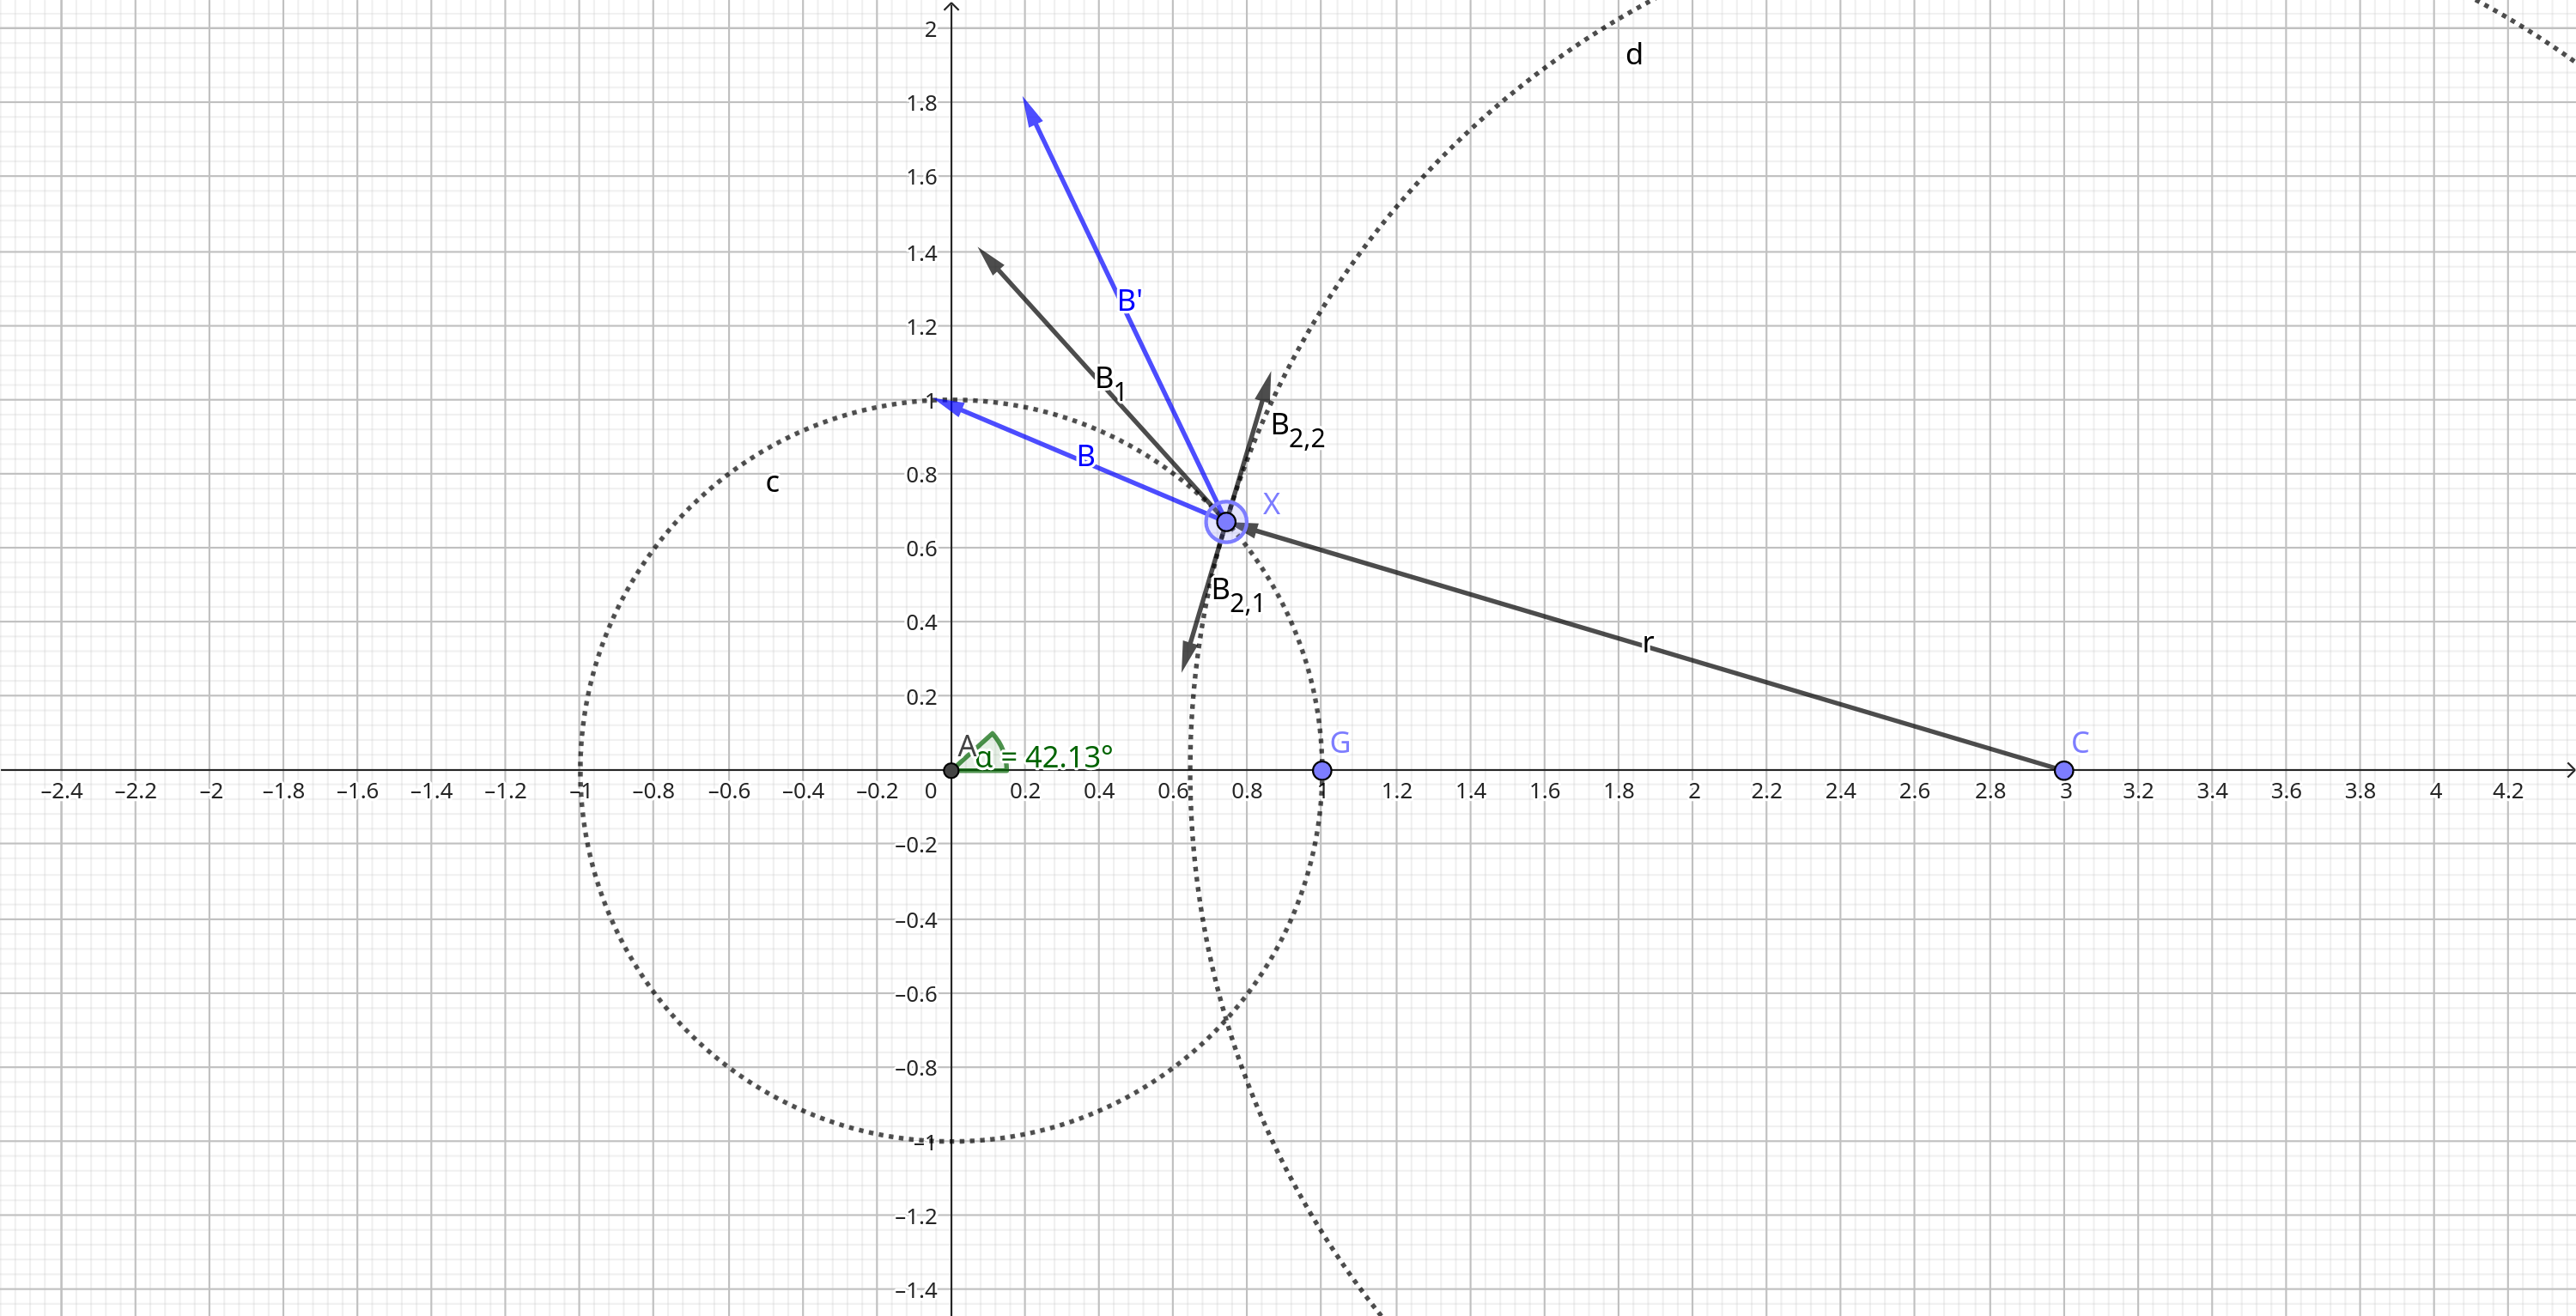
\includegraphics[width=0.95\textwidth]{2-fig.png}
  \caption{Konstrukce úlohy}
  \label{fig:1}
\end{figure}

\begin{figure}
  \centering
  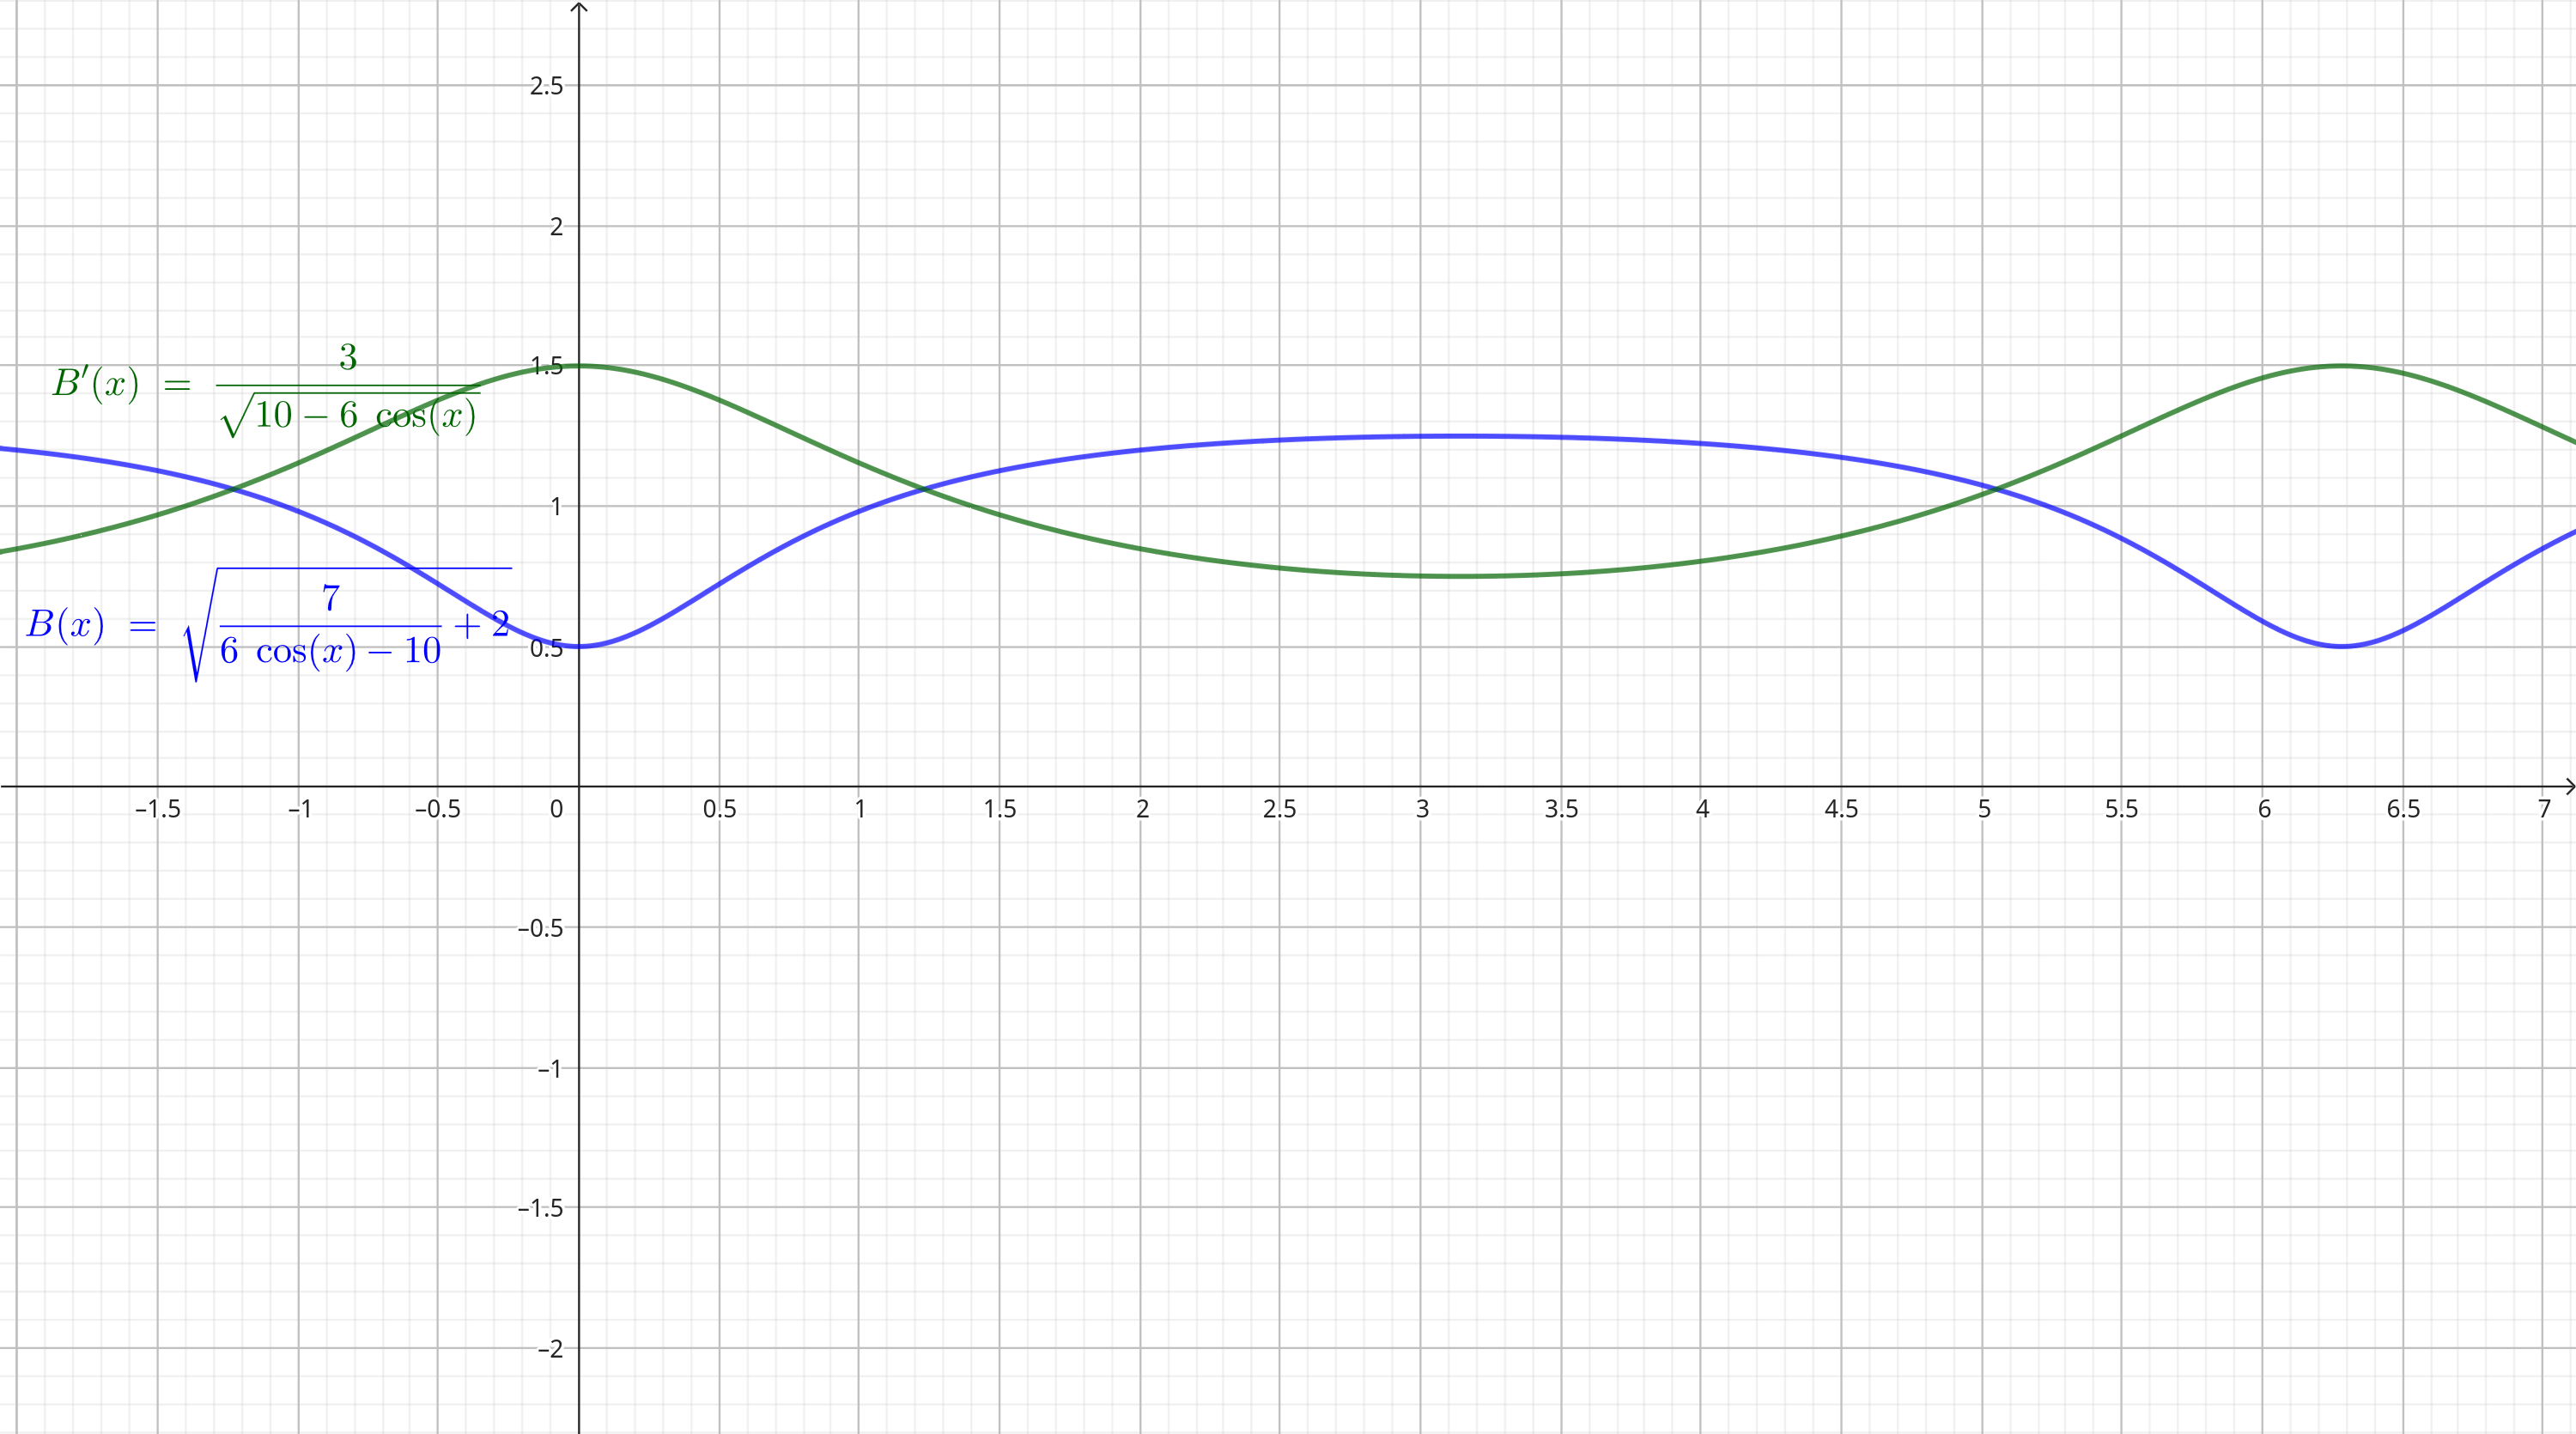
\includegraphics[width=0.95\textwidth]{2-fig2.png}
  \caption{Graf funkcí}
  \label{fig:2}
\end{figure}

\end{document}
